% Urban Heat and Health in Johannesburg - PhD Protocol Presentation
% Craig Parker - April 11, 2025
\documentclass[aspectratio=169]{beamer}

% Theme and color settings
\usetheme{Madrid}
\useoutertheme{infolines}
\usecolortheme{beaver}
\setbeamertemplate{navigation symbols}{}
\setbeamertemplate{headline}{}
\setbeamertemplate{footline}[frame number]

% Enhanced typography and design packages
\usepackage{graphicx}
\usepackage{booktabs}
\usepackage{amsmath}
\usepackage{amssymb}
\usepackage{textcomp}
\usepackage{xcolor}
\usepackage{tikz}
\usepackage{adjustbox}
\usepackage{ragged2e}
\usepackage{fontawesome5}
\usepackage[skins]{tcolorbox}
\usepackage{lmodern}          % Modern font
\usepackage{microtype}        % Typography improvements
\usepackage{multicol}         % Better column control
\usepackage{enumitem}         % Better list control
\usepackage{pgfplots}         % Better plots
\usepackage{colortbl}         % Table color control
\usepackage[framemethod=tikz]{mdframed} % Better frames
\usepackage[utf8]{inputenc}   % Added to handle Unicode characters

% Enhanced color scheme
\definecolor{witsteal}{RGB}{0, 151, 169}
\definecolor{witsyellow}{RGB}{255, 202, 5}
\definecolor{witsdark}{RGB}{0, 90, 101}
\definecolor{witslight}{RGB}{219, 242, 244}
\definecolor{witsaccent}{RGB}{255, 127, 42} % Orange accent

% Apply colors to beamer elements
\setbeamercolor{frametitle}{bg=witsteal,fg=white}
\setbeamercolor{title}{bg=witsdark,fg=white}
\setbeamercolor{structure}{fg=witsteal}
\setbeamercolor{itemize item}{fg=witsteal}
\setbeamercolor{itemize subitem}{fg=witsteal}
\setbeamercolor{block title}{bg=witsteal,fg=white}
\setbeamercolor{block body}{bg=witslight,fg=black}
\setbeamercolor{section in toc}{fg=witsteal}
\setbeamercolor{description item}{fg=witsdark}
\setbeamercolor{caption name}{fg=witsteal}

% Set paths for images
\graphicspath{{images/}}

% Custom bullet point style
\setbeamertemplate{itemize item}{\color{witsteal}$\blacktriangleright$}
\setbeamertemplate{itemize subitem}{\color{witsteal}$\bullet$}

% Custom commands for consistent styling
\newcommand{\highlight}[1]{\colorbox{witsyellow!30}{#1}}
\newcommand{\concept}[1]{\textcolor{witsteal}{\textbf{#1}}}
\newcommand{\statistic}[1]{\textcolor{witsaccent}{\textbf{#1}}}
\newcommand{\insighttitle}[1]{\textcolor{witsdark}{\textbf{\Large #1}}}

% Custom block styles
\newtcolorbox{infobox}[1][]{
  enhanced,
  colback=witslight,
  colframe=witsteal,
  boxrule=1pt,
  fonttitle=\bfseries,
  coltitle=white,
  attach boxed title to top left={yshift=-2mm, xshift=3mm},
  boxed title style={colback=witsteal},
  title=#1
}

\newtcolorbox{impactbox}[1][]{
  enhanced,
  colback=witsyellow!10,
  colframe=witsyellow!70!orange,
  boxrule=1pt,
  fonttitle=\bfseries,
  coltitle=black,
  attach boxed title to top left={yshift=-2mm, xshift=3mm},
  boxed title style={colback=witsyellow},
  title=#1
}

\newtcolorbox{keypoint}{
  enhanced,
  colback=witsaccent!10,
  colframe=witsaccent,
  boxrule=0.5pt,
  sharp corners,
  left=5pt,
  right=5pt,
  top=5pt,
  bottom=5pt
}

% Section transitions
\AtBeginSection[]
{
  \begingroup
  \setbeamercolor{background canvas}{bg=witsdark}
  \begin{frame}[plain]
    \vspace{2cm}
    \begin{center}
      \textcolor{white}{\Huge\insertsectionhead}
      \vspace{0.8cm}
      
      \textcolor{witsyellow}{\rule{0.8\textwidth}{2pt}}
    \end{center}
  \end{frame}
  \endgroup
}

% Title information
\title[Urban Heat \& Health]{Urban Heat and Health in Johannesburg}
\subtitle{A Multidimensional Analysis of Vulnerability, Explanatory Modelling, and Predictive Outcomes}
\author[Craig Parker]{Craig Parker, MSc, MM-PDM, BS}
\institute[Wits University]{School of Public Health\\University of the Witwatersrand}
\date{April 11, 2025}

\begin{document}

% Custom title page
\begingroup
\setbeamercolor{background canvas}{bg=witsdark}
\begin{frame}[plain]
    \begin{center}
        \vspace{-0.8cm}  % Reduced top margin
        \textcolor{white}{\Huge\textbf{Urban Heat and Health}}
        \vspace{0.2cm}  % Reduced spacing
        
        \textcolor{white}{\Large in Johannesburg}
        \vspace{0.1cm}  % Reduced spacing
        
        \textcolor{witsyellow}{\rule{0.7\textwidth}{2pt}}
        \vspace{0.3cm}  % Reduced spacing
        
        \begin{columns}[T,totalwidth=\textwidth]
            \begin{column}{0.68\textwidth}  % Slightly adjusted column width
                \textcolor{white}{\large A Multidimensional Analysis of Vulnerability,}\\
                \textcolor{white}{\large Explanatory Modelling, and Predictive Outcomes}
                \vspace{1cm}  % Reduced spacing
                
                \textcolor{white}{\normalsize Craig Parker, MSc, MM-PDM, BS}\\
                \textcolor{witslight}{\normalsize School of Public Health}\\
                \textcolor{witslight}{\normalsize University of the Witwatersrand}
                \vspace{0.2cm}  % Reduced spacing
                
                \textcolor{witsaccent}{April 11, 2025}
                \vspace{0.3cm}  % Reduced spacing
                
                \textcolor{witslight}{\small PhD Protocol Presentation}
            \end{column}
            \begin{column}{0.28\textwidth}  % Slightly adjusted column width
                \vspace{-0.5cm}  % Adjust image position
                \includegraphics[width=\textwidth]{concept_note (1).png}
            \end{column}
        \end{columns}
    \end{center}
\end{frame}
\endgroup

\begin{frame}
    \frametitle{Why This Research Matters}
    
    \begin{center}
        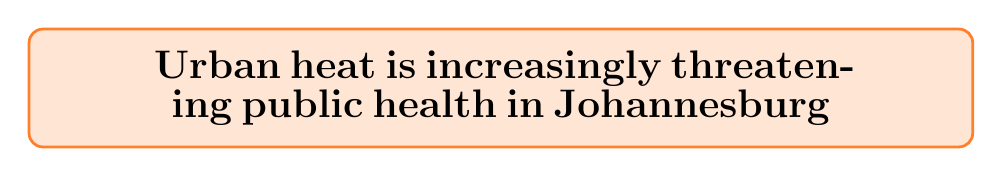
\begin{tikzpicture}
            \node[fill=witsaccent!20, text width=\textwidth-20pt, align=center, rounded corners=5pt, 
                  draw=witsaccent, line width=1pt, inner sep=8pt] {
                \textbf{\Large Urban heat is increasingly threatening public health in Johannesburg}
            };
        \end{tikzpicture}
    \end{center}
    
    \vspace{0.3cm}
    \begin{columns}[T]
        \begin{column}{0.48\textwidth}
            \begin{infobox}[Human Impact]
                \begin{itemize}[leftmargin=*, itemsep=6pt]
                    \item \statistic{0.9\%} mortality increase per 1°C above 18.7°C
                    \item \statistic{2.1\%} increase for elderly residents
                    \item Record temperatures reaching \statistic{38°C}
                \end{itemize}
            \end{infobox}
        \end{column}
        \begin{column}{0.48\textwidth}
            \begin{infobox}[Spatial Inequality]
                \begin{itemize}[leftmargin=*, itemsep=6pt]
                    \item Townships up to \statistic{6°C} hotter than wealthy areas
                    \item Informal housing \statistic{15°C} higher indoor temperatures
                    \item Minimal green infrastructure in vulnerable areas
                \end{itemize}
            \end{infobox}
        \end{column}
    \end{columns}
    
    \vspace{0.3cm}
    \begin{keypoint}
        \centering
        \textbf{This research will transform how African cities understand and address heat vulnerability}
    \end{keypoint}
\end{frame}

\begin{frame}
    \frametitle{Presentation Overview}
    
    \vspace{0.3cm}
    \begin{columns}[T]
        \begin{column}{0.48\textwidth}
            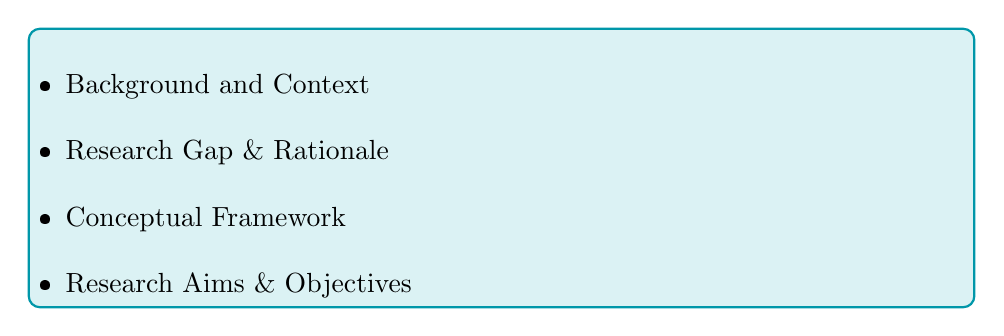
\begin{tikzpicture}
                \node[fill=witslight, draw=witsteal, thick, text width=\textwidth-10pt, rounded corners] {
                    \begin{itemize}[leftmargin=*, itemsep=8pt]
                        \item Background and Context
                        \item Research Gap \& Rationale
                        \item Conceptual Framework
                        \item Research Aims \& Objectives
                    \end{itemize}
                };
            \end{tikzpicture}
        \end{column}
        \begin{column}{0.48\textwidth}
            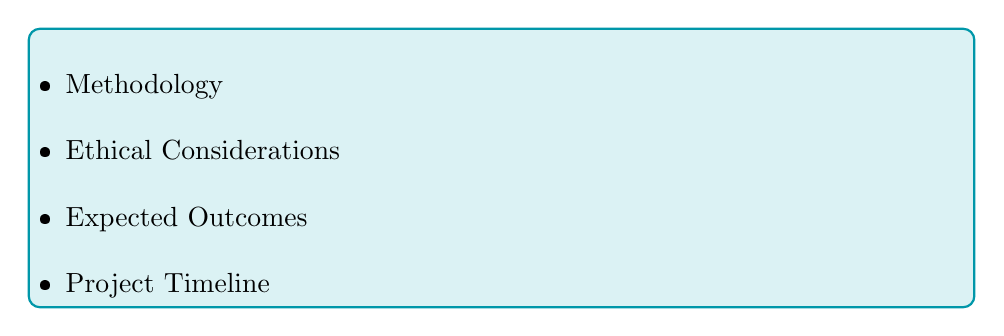
\begin{tikzpicture}
                \node[fill=witslight, draw=witsteal, thick, text width=\textwidth-10pt, rounded corners] {
                    \begin{itemize}[leftmargin=*, itemsep=8pt]
                        \item Methodology
                        \item Ethical Considerations
                        \item Expected Outcomes
                        \item Project Timeline
                    \end{itemize}
                };
            \end{tikzpicture}
        \end{column}
    \end{columns}
    
    \vspace{0.8cm}
    \begin{center}
        \begin{tikzpicture}
            \node[fill=witsteal!15, draw=witsteal, rounded corners, text width=9cm, align=center, inner sep=15pt] {
                \textbf{Research Journey:} \\
                Understanding → Explaining → Predicting → Acting
            };
        \end{tikzpicture}
    \end{center}
\end{frame}

% SECTION: Background and Context
\section{Background and Context}

\begin{frame}
    \frametitle{Climate Change and Heat-Health Impacts}
    
    \begin{columns}[T]
        \begin{column}{0.55\textwidth}
            \begin{itemize}[leftmargin=*, itemsep=8pt]
                \item Global warming exceeding \statistic{1.2°C} since pre-industrial era
                \item Urban areas experiencing amplified effects
                \item \textbf{Johannesburg impacts:}
                \begin{itemize}[itemsep=6pt]
                    \item Record \statistic{38°C} (2016)
                    \item Mortality increases \statistic{0.9\%} per 1°C above 18.7°C
                    \item Elderly: \statistic{2.1\%} increase per 1°C
                \end{itemize}
            \end{itemize}
            
            \begin{tikzpicture}
                \node[fill=witsaccent!15, text width=\textwidth-10pt, align=center, rounded corners, inner sep=8pt] {
                    \textbf{Urban temperatures up to 8°C warmer than surrounding rural areas}
                };
            \end{tikzpicture}
        \end{column}
        \begin{column}{0.42\textwidth}
            \begin{figure}
                \includegraphics[width=\textwidth]{global_temp.png}
                \caption{\small Global temperature trends showing accelerating warming patterns}
            \end{figure}
        \end{column}
    \end{columns}
\end{frame}

\begin{frame}
    \frametitle{Climate Projections for Johannesburg}
    
    \begin{columns}[T]
        \begin{column}{0.55\textwidth}
            \begin{impactbox}[By 2050 (High-Emissions Scenario)]
                \begin{itemize}[leftmargin=*, itemsep=6pt]
                    \item \statistic{$\approx$ 2°C} warming
                    \item Hot nights ($>$20°C) to \statistic{quadruple}
                    \item \statistic{3-4} additional weeks of very hot days
                \end{itemize}
            \end{impactbox}
            \vspace{0.4cm}
            \begin{itemize}[leftmargin=*, itemsep=8pt]
                \item By 2100: potential \statistic{6-7°C} increase
                \item IPCC: Beyond +2°C, heat-related mortality in Africa will sharply rise
            \end{itemize}
        \end{column}
        \begin{column}{0.42\textwidth}
            \begin{figure}
                \includegraphics[width=\textwidth]{max_temp.png}
                \caption{\small Johannesburg maximum temperature projections showing alarming upward trends}
            \end{figure}
        \end{column}
    \end{columns}
    
    \vspace{0.3cm}
    \begin{keypoint}
        \centering
        Heat extremes that were once rare will become commonplace, with profound implications for public health
    \end{keypoint}
\end{frame}

\begin{frame}
    \frametitle{Urban Context and Legacy of Apartheid Planning}
    
    \begin{columns}[T]
        \begin{column}{0.55\textwidth}
            \begin{itemize}[leftmargin=*, itemsep=8pt]
                \item Johannesburg: 5.87 million people, 1753m elevation
                \item Legacy of apartheid spatial planning:
                \begin{itemize}[itemsep=6pt]
                    \item \concept{Wealthy areas:} Abundant green spaces, tree canopy
                    \item \concept{Townships:} Dense settlements, minimal vegetation, dark surfaces
                \end{itemize}
            \end{itemize}
            
            \begin{tcolorbox}[colback=witsteal!10, colframe=witsteal, title=Temperature Disparities]
                \begin{itemize}[leftmargin=*, itemsep=6pt]
                    \item Townships \statistic{$\approx$ 6°C} hotter than surrounding areas
                    \item Indoor temperatures in informal settlements up to \statistic{15°C} higher than ambient
                    \item Extreme vulnerability for elderly and chronically ill
                \end{itemize}
            \end{tcolorbox}
        \end{column}
        \begin{column}{0.42\textwidth}
            \begin{figure}
                \includegraphics[width=\textwidth]{heat_stress.png}
                \caption{\small Thermal imagery showing stark temperature differences between historically white suburbs and townships}
            \end{figure}
        \end{column}
    \end{columns}
\end{frame}

% SECTION: Research Gap and Rationale
\section{Research Gap and Rationale}

\begin{frame}
    \frametitle{Research Gap and Rationale}
    
    \begin{columns}[T]
        \begin{column}{0.48\textwidth}
            \begin{tcolorbox}[colback=witsteal!10, colframe=witsteal, title=Current Research Limitations]
                \begin{itemize}[leftmargin=*, itemsep=6pt]
                    \item Limited African urban heat studies
                    \item Siloed disciplinary approaches
                    \item Models developed in Global North with limited applicability
                    \item African-specific urban challenges understudied
                \end{itemize}
            \end{tcolorbox}
        \end{column}
        
        \begin{column}{0.48\textwidth}
            \begin{tcolorbox}[colback=witsteal!10, colframe=witsteal, title=Johannesburg's Unique Challenges]
                \begin{itemize}[leftmargin=*, itemsep=6pt]
                    \item Historical spatial disparities
                    \item Complex disease burden (HIV, TB, NCDs)
                    \item Accelerating climate impacts
                    \item Informal housing predominance
                \end{itemize}
            \end{tcolorbox}
        \end{column}
    \end{columns}
    
    \vspace{0.5cm}
    \begin{center}
        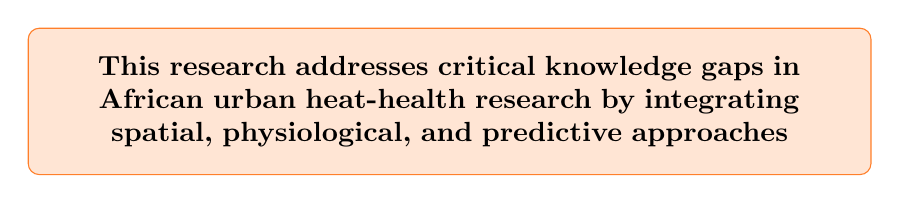
\begin{tikzpicture}
            \node[fill=witsaccent!20, text width=10cm, align=center, rounded corners, draw=witsaccent, inner sep=10pt] {
                \textbf{This research addresses critical knowledge gaps in African urban heat-health research by integrating spatial, physiological, and predictive approaches}
            };
        \end{tikzpicture}
    \end{center}
\end{frame}

% SECTION: Conceptual Framework
\section{Conceptual Framework}

\begin{frame}
    \frametitle{Heat Vulnerability Framework}
    
    \begin{columns}[T]
        \begin{column}{0.55\textwidth}
            \insighttitle{Three Interconnected Dimensions:}
            \vspace{0.3cm}
            
            \begin{description}[leftmargin=!, labelwidth=\widthof{\bfseries Adaptive Capacity}]
                \item[\concept{Exposure}] Heat intensity and duration
                \begin{itemize}[itemsep=4pt]
                    \item Dense urban areas: Up to \statistic{5°C} higher
                    \item Nighttime retention in informal settlements
                \end{itemize}
                \item[\concept{Sensitivity}] Population susceptibility
                \begin{itemize}[itemsep=4pt]
                    \item Health status, chronic conditions
                    \item Age extremes, pregnancy
                \end{itemize}
                \item[\concept{Adaptive Capacity}] Resources for coping
                \begin{itemize}[itemsep=4pt]
                    \item Access to cooling, healthcare, support
                    \item Economic resources, social networks
                \end{itemize}
            \end{description}
        \end{column}
        \begin{column}{0.4\textwidth}
            \begin{figure}
                \includegraphics[width=\textwidth]{HVI.png}
                \caption{\small Heat Vulnerability Index components showing the interplay between physical, social, and health factors}
            \end{figure}
        \end{column}
    \end{columns}
    
    \vspace{0.3cm}
    \begin{keypoint}
        \centering
        Vulnerability is not just about temperature—it's about the complex interaction of exposure, sensitivity, and adaptive capacity
    \end{keypoint}
\end{frame}

% SECTION: Research Aims & Objectives
\section{Research Aims \& Objectives}

\begin{frame}
    \frametitle{Primary Aim and Research Objectives}
    
    \begin{center}
        
\begin{tikzpicture}
            \node[fill=witsdark, text=white, text width=\textwidth-40pt, align=center, rounded corners] {
                \textbf{\Large Primary Aim}
            };
        \end{tikzpicture}
        
        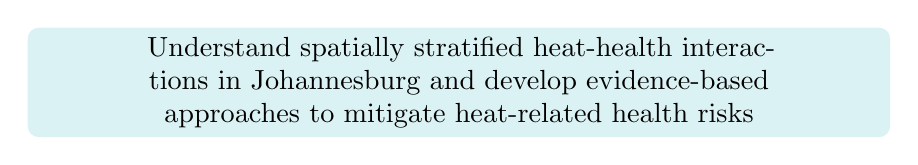
\begin{tikzpicture}
            \node[fill=witslight, text width=\textwidth-40pt, align=center, rounded corners] {
                Understand spatially stratified heat-health interactions in Johannesburg and develop evidence-based approaches to mitigate heat-related health risks
            };
        \end{tikzpicture}
    \end{center}
    
    \vspace{0.3cm}
    \textbf{\large Three Interconnected Objectives:}
    
    \begin{figure}
        \centering
        \begin{tikzpicture}[node distance=1.2cm]
            \node[draw, rounded corners, fill=witsteal!70, text=white, text width=7cm, align=center] (aim) {\textbf{Understanding Heat-Health Interactions}};
            
            \node[draw, rounded corners, below of=aim, fill=witsteal!20, text width=3cm, align=center] (obj1) {\textbf{1. Vulnerability Mapping}\\(Descriptive)};
            
            \node[draw, rounded corners, below of=obj1, fill=witsteal!30, text width=3cm, align=center] (obj2) {\textbf{2. Heat-Health Dynamics}\\(Explanatory)};
            
            \node[draw, rounded corners, below of=obj2, fill=witsteal!40, text width=3cm, align=center] (obj3) {\textbf{3. Predictive Modeling}\\(Predictive)};
            
            \draw[->, thick, witsteal] (aim) -- (obj1);
            \draw[->, thick, witsteal] (obj1) -- (obj2);
            \draw[->, thick, witsteal] (obj2) -- (obj3);
            
            \node[right=0.2cm of obj1, text width=4cm, align=left] {\footnotesize\textit{Where are the vulnerable populations?}};
            \node[right=0.2cm of obj2, text width=4cm, align=left] {\footnotesize\textit{Why are they vulnerable?}};
            \node[right=0.2cm of obj3, text width=4cm, align=left] {\footnotesize\textit{How will risks evolve?}};
        \end{tikzpicture}
    \end{figure}
\end{frame}

\begin{frame}
    \frametitle{Objective 1: Heat Vulnerability Mapping}
    
    \begin{columns}[T]
        \begin{column}{0.55\textwidth}
            \textbf{\large Key Activities:}
            \begin{itemize}[leftmargin=*, itemsep=6pt]
                \item Comprehensive spatial vulnerability assessment
                \item Integration of multiple data sources:
                \begin{itemize}[itemsep=4pt]
                    \item \concept{Environmental:} Satellite imagery, temperature networks
                    \item \concept{Socioeconomic:} Housing quality, infrastructure access
                    \item \concept{Health:} Disease prevalence, healthcare access
                \end{itemize}
                \item Advanced spatial statistical analysis
            \end{itemize}
            
            \vspace{-0.2cm} % Reduce space before the box to move it up
            \begin{impactbox}[Expected Outcomes]
                \begin{itemize}[leftmargin=*, itemsep=6pt]
                    \item High-resolution vulnerability maps
                    \item Identification of vulnerability hotspots
                    \item Quantification of spatial vulnerability patterns
                    \item Evidence base for targeting interventions
                \end{itemize}
            \end{impactbox}
        \end{column}
        \begin{column}{0.42\textwidth}
            \begin{figure}
                \includegraphics[width=\textwidth]{temp_distribution.png}
                \caption{\small Heat Vulnerability Index distribution showing stark spatial disparities between neighborhoods}
            \end{figure}
        \end{column}
    \end{columns}
\end{frame}

\begin{frame}
    \frametitle{Objective 2: Heat-Health Dynamics Methodology}
    
    \begin{columns}[T]
        \begin{column}{0.55\textwidth}
            \textbf{\large Clinical-Computational Approach:}
            \begin{itemize}[leftmargin=*, itemsep=3pt]
                \item Validated mechanistic pathway modeling
                \item Multi-system physiological analysis
                \item Temporal dynamics analysis
            \end{itemize}
            
            \textbf{Distributed Lag Model}
            {\small $g[E(Y_t)] = \alpha + \sum_{l=0}^{L}f(x_{t-l}, l)$}
            
            \textbf{\large Machine Learning Approaches:}
            \begin{itemize}[leftmargin=*, itemsep=3pt]
                \item Random Forests for feature importance
                \item XGBoost with SHAP values for explanation
                \item LIME explanations for model interpretability
            \end{itemize}
        \end{column}
        \begin{column}{0.42\textwidth}
            \begin{figure}
                \includegraphics[width=\textwidth]{mechanisms-inflammatory.drawio (2).png}
                \caption{\small Inflammatory pathways affected by heat stress}
            \end{figure}
            
            \vspace{-0.2cm}
            \begin{impactbox}[Key Advantages]
                \begin{itemize}[leftmargin=*, itemsep=2pt]
                    \item Explainable AI approaches
                    \item Identification of causal links
                    \item Clinically actionable insights
                \end{itemize}
            \end{impactbox}
        \end{column}
    \end{columns}
\end{frame}

\begin{frame}
    \frametitle{Objective 3: Heat-Health Prediction Modeling}
    
    \begin{columns}[T]
        \begin{column}{0.55\textwidth}
            \textbf{\large Key Activities:}
            \begin{itemize}[leftmargin=*, itemsep=4pt]
                \item Development of predictive frameworks for heat-related outcomes
                \item Stratified predictions by:
                \begin{itemize}[itemsep=2pt]
                    \item Geographic location
                    \item Demographic characteristics
                    \item Housing conditions
                \end{itemize}
                \item Identification of risk conditions at specific temperature thresholds
                \item Focus on vulnerable populations:
                \begin{itemize}[itemsep=2pt]
                    \item Elderly residents
                    \item People with pre-existing conditions
                    \item Those with limited adaptive capacity
                \end{itemize}
            \end{itemize}
        \end{column}
        \begin{column}{0.42\textwidth}
            \begin{impactbox}[Model Applications]
                \begin{itemize}[leftmargin=*, itemsep=3pt]
                    \item Early warning systems
                    \item Healthcare resource allocation
                    \item Heat action plan development
                    \item Spatial targeting of interventions
                    \item Climate adaptation policy
                \end{itemize}
            \end{impactbox}
            
            \vspace{-0.2cm}
            \begin{figure}
                \includegraphics[width=\textwidth]{mechanisms-Renal.drawio (2).png}
                \caption{\small Renal pathways affected by heat stress}
            \end{figure}
        \end{column}
    \end{columns}
\end{frame}

\begin{frame}
    \frametitle{Multi-method Approach and Data Sources}
    
    \begin{columns}[T]
        \begin{column}{0.48\textwidth}
            \textbf{\large Methodological Approach:}
            \begin{itemize}[leftmargin=*, itemsep=6pt]
                \item Advanced geospatial analysis
                \item Statistical modeling
                \item Machine learning techniques
            \end{itemize}
            
            \textbf{\large Sample Size:}
            \begin{itemize}[leftmargin=*, itemsep=6pt]
                \item All 135 Johannesburg wards (complete coverage)
                \item 5,000-7,000 clinical records
                \item >80\% power for detecting relevant effects
            \end{itemize}
        \end{column}
        \begin{column}{0.48\textwidth}
            \textbf{\large Key Data Sources:}
            \begin{table}[h]
                \small
                \begin{tabular}{p{2.5cm}p{3cm}}
                    \toprule
                    \textbf{Category} & \textbf{Sources} \\
                    \midrule
                    Health Data & Clinical trials \& cohort studies (2000-2022) \\
                    \addlinespace
                    Environmental Data & Landsat 8, Sentinel-2, ERA5, MODIS LST \\
                    \addlinespace
                    Socioeconomic & Gauteng City-Region Observatory, QoL Surveys \\
                    \bottomrule
                \end{tabular}
            \end{table}
            
            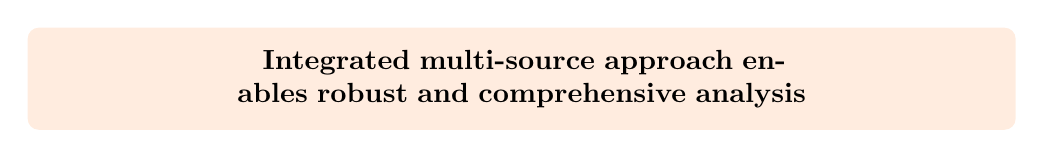
\begin{tikzpicture}
                \node[fill=witsaccent!15, text width=\columnwidth-4pt, align=center, rounded corners, inner sep=8pt] {
                    \textbf{Integrated multi-source approach enables robust and comprehensive analysis}
                };
            \end{tikzpicture}
        \end{column}
    \end{columns}
\end{frame}

\begin{frame}
    \frametitle{Objective 1: Vulnerability Mapping Methodology}
    
    \begin{columns}[T]
        \begin{column}{0.55\textwidth}
            \textbf{\large Analytical Approach:}
            \begin{itemize}[leftmargin=*, itemsep=3pt]
                \item Principal Component Analysis for Heat Vulnerability Index
                \item Geographically Weighted PCA for spatial non-stationarity
                
                $X_i = V_i \Lambda_i V_i^T + \varepsilon_i$
                
                \item Spatial clustering (LISA)
                
                $I_i = z_i\sum_{j}w_{ij}z_j$
                
                \item Geographic de-identification to ensure privacy
            \end{itemize}
        \end{column}
        \begin{column}{0.42\textwidth}
            \begin{figure}
                \includegraphics[width=\textwidth]{seasonal_heat.png}
                \caption{\small Urban heat patterns showing correlation with socioeconomic variables}
            \end{figure}
            
            \vspace{-0.2cm}
            \begin{infobox}[Privacy Protection]
                \begin{itemize}[leftmargin=*, itemsep=2pt]
                    \item Data aggregation by ward
                    \item Geographic masking
                    \item Statistical disclosure control
                \end{itemize}
            \end{infobox}
        \end{column}
    \end{columns}
\end{frame}

\begin{frame}
    \frametitle{Objective 2: Heat-Health Dynamics Methodology}
    
    \begin{columns}[T]
        \begin{column}{0.55\textwidth}
            \textbf{\large Clinical-Computational Approach:}
            \begin{itemize}[leftmargin=*, itemsep=3pt]
                \item Validated mechanistic pathway modeling
                \item Multi-system physiological analysis
                \item Temporal dynamics analysis
            \end{itemize}
            
            \textbf{Distributed Lag Model}
            {\small $g[E(Y_t)] = \alpha + \sum_{l=0}^{L}f(x_{t-l}, l)$}
            
            \textbf{\large Machine Learning Approaches:}
            \begin{itemize}[leftmargin=*, itemsep=3pt]
                \item Random Forests for feature importance
                \item XGBoost with SHAP values for explanation
                \item LIME explanations for model interpretability
            \end{itemize}
        \end{column}
        \begin{column}{0.42\textwidth}
            \begin{figure}
                \includegraphics[width=\textwidth]{mechanisms-inflammatory.drawio (2).png}
                \caption{\small Inflammatory pathways affected by heat stress}
            \end{figure}
            
            \vspace{-0.2cm}
            \begin{impactbox}[Key Advantages]
                \begin{itemize}[leftmargin=*, itemsep=2pt]
                    \item Explainable AI approaches
                    \item Identification of causal links
                    \item Clinically actionable insights
                \end{itemize}
            \end{impactbox}
        \end{column}
    \end{columns}
\end{frame}

\begin{frame}
    \frametitle{Objective 3: Predictive Modeling Methodology}
    
    \begin{columns}[T]
        \begin{column}{0.55\textwidth}
            \textbf{\large Modeling Framework:}
            \begin{itemize}[leftmargin=*, itemsep=6pt]
                \item Ensemble machine learning approaches
                \item Time-series cross-validation
                \item Stratified risk profiles
            \end{itemize}
            
            \textbf{Key Equations}
            \begin{align*}
            L(\phi) &= \sum_{i=1}^{n}l(y_i, \hat{y}_i) + \sum_{k=1}^{K}\Omega(f_k) \\
            \text{AUC-ROC} &= \int_{0}^{1} \text{TPR}(\text{FPR}^{-1}(t))dt
            \end{align*}
        \end{column}
        \begin{column}{0.42\textwidth}
            \textbf{\large Temporal Analysis:}
            \begin{table}[h]
                \small
                \begin{tabular}{p{2cm}p{2.8cm}}
                    \toprule
                    \textbf{Scale} & \textbf{Health Outcomes} \\
                    \midrule
                    Immediate & Cardiovascular, renal \\
                    (0-24h) & function markers \\
                    \addlinespace
                    Short-term & Inflammatory markers, \\
                    (1-7d) & metabolic changes \\
                    \addlinespace
                    Medium-term & Chronic conditions, \\
                    (7-30d) & adaptation responses \\
                    \bottomrule
                \end{tabular}
            \end{table}
            
            \begin{infobox}[Model Evaluation]
                \begin{itemize}[leftmargin=*, itemsep=4pt]
                    \item Nested cross-validation
                    \item Out-of-time validation
                    \item Performance by subgroups
                \end{itemize}
            \end{infobox}
        \end{column}
    \end{columns}
\end{frame}

\begin{frame}
    \frametitle{Ethical Considerations}
    
    \begin{columns}[T]
        \begin{column}{0.32\textwidth}
            \begin{infobox}[Regulatory Compliance]
                \begin{itemize}[leftmargin=*, itemsep=4pt]
                    \item Wits HREC (ref 220606)
                    \item US HHS regulations (45 CFR 46)
                    \item South Africa's POPIA (2013)
                \end{itemize}
            \end{infobox}
        \end{column}
        \begin{column}{0.32\textwidth}
            \begin{infobox}[Data Privacy]
                \begin{itemize}[leftmargin=*, itemsep=4pt]
                    \item Data minimization
                    \item Secure restricted access
                    \item Geographic jittering
                    \item AES-256 encryption
                \end{itemize}
            \end{infobox}
        \end{column}
        \begin{column}{0.32\textwidth}
            \begin{infobox}[Secondary Data Usage]
                \begin{itemize}[leftmargin=*, itemsep=4pt]
                    \item Verification of consent
                    \item Contractual guarantees
                    \item Institutional compliance
                \end{itemize}
            \end{infobox}
        \end{column}
    \end{columns}
    
    \vspace{0.6cm}
    \begin{center}
        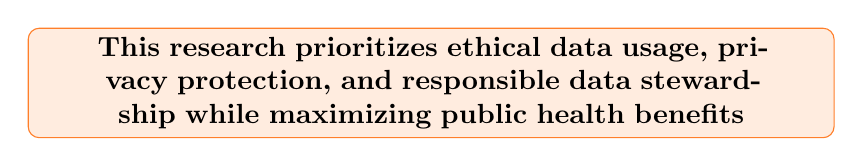
\begin{tikzpicture}
            \node[fill=witsaccent!15, text width=10cm, align=center, rounded corners, draw=witsaccent] {
                \textbf{This research prioritizes ethical data usage, privacy protection, and responsible data stewardship while maximizing public health benefits}
            };
        \end{tikzpicture}
    \end{center}
\end{frame}

\begin{frame}
    \frametitle{Expected Outcomes and Impact}
    
    \begin{columns}[T]
        \begin{column}{0.48\textwidth}
            \begin{infobox}[Public Health Practice]
                \begin{itemize}[leftmargin=*, itemsep=6pt]
                    \item Targeted vulnerable population interventions
                    \item Precise clinical risk stratification
                    \item Proactive outreach protocols
                \end{itemize}
            \end{infobox}
            
            \begin{infobox}[Urban Planning]
                \begin{itemize}[leftmargin=*, itemsep=6pt]
                    \item Evidence-based cooling strategies
                    \item Green infrastructure priority areas
                    \item Resilient building designs
                \end{itemize}
            \end{infobox}
        \end{column}
        \begin{column}{0.48\textwidth}
            \begin{infobox}[Climate Adaptation Policy]
                \begin{itemize}[leftmargin=*, itemsep=6pt]
                    \item Transferable methods for African cities
                    \item Comprehensive heat-health action plans
                    \item Cross-sector collaboration models
                \end{itemize}
            \end{infobox}
            
            \begin{infobox}[Community Resilience]
                \begin{itemize}[leftmargin=*, itemsep=6pt]
                    \item Locally-accessible information
                    \item Community-based monitoring
                    \item Targeted intervention strategies
                \end{itemize}
            \end{infobox}
        \end{column}
    \end{columns}
\end{frame}

\begin{frame}
    \frametitle{Project Timeline}
    
    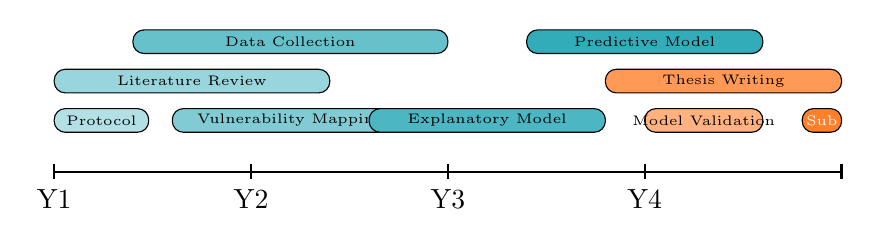
\begin{tikzpicture}
        \draw[thick] (0,0) -- (10,0);
        \foreach \x in {0,2.5,5,7.5,10}
            \draw[thick] (\x,0.1) -- (\x,-0.1);
        
        \node[below] at (0,-0.1) {Y1};
        \node[below] at (2.5,-0.1) {Y2};
        \node[below] at (5,-0.1) {Y3};
        \node[below] at (7.5,-0.1) {Y4};
        \node[below] at (10,-0.1) {};
        
        % Timeline bars
        \draw[fill=witsteal!30, rounded corners] (0,0.5) rectangle (1.2,0.8) node[midway] {\tiny Protocol};
        \draw[fill=witsteal!40, rounded corners] (0,1.0) rectangle (3.5,1.3) node[midway] {\tiny Literature Review};
        \draw[fill=witsteal!50, rounded corners] (1.5,0.5) rectangle (4.5,0.8) node[midway] {\tiny Vulnerability Mapping};
        \draw[fill=witsteal!60, rounded corners] (1.0,1.5) rectangle (5.0,1.8) node[midway] {\tiny Data Collection};
        \draw[fill=witsteal!70, rounded corners] (4.0,0.5) rectangle (7.0,0.8) node[midway] {\tiny Explanatory Model};
        \draw[fill=witsteal!80, rounded corners] (6.0,1.5) rectangle (9.0,1.8) node[midway] {\tiny Predictive Model};
        \draw[fill=witsaccent!60, rounded corners] (7.5,0.5) rectangle (9.0,0.8) node[midway] {\tiny Model Validation};
        \draw[fill=witsaccent!80, rounded corners] (7.0,1.0) rectangle (10,1.3) node[midway] {\tiny Thesis Writing};
        \draw[fill=witsaccent, rounded corners] (9.5,0.5) rectangle (10,0.8) node[midway, text=white] {\tiny Sub};
    \end{tikzpicture}
    
    \vspace{0.6cm}
    \begin{tcolorbox}[colback=witslight, colframe=witsteal, title=Key Timeline Information]
        \begin{itemize}[leftmargin=*, itemsep=6pt]
            \item 36-month research project with four phases
            \item Critical milestones: Protocol (M3), Data collection (M9), Mapping (M18), Validation (M30), Submission (M36)
        \end{itemize}
    \end{tcolorbox}
\end{frame}

\begin{frame}
    \frametitle{Supervision Framework}
    
    \textbf{\large Multidisciplinary Supervisory Team}
    \begin{table}[h]
        \small
        \begin{tabular}{p{2.5cm}p{2.5cm}p{3.5cm}}
            \toprule
            \textbf{Supervisor} & \textbf{Affiliation} & \textbf{Expertise} \\
            \midrule
            Dr. Admire Chikandiwa & Wits University & Clinical epidemiology \\
            \addlinespace
            Prof. Matthew Chersich & Trinity/Wits & Climate and health \\
            \addlinespace
            Prof. Akbar Waljee & Michigan & Statistical modeling, ML \\
            \addlinespace
            Dr. Christopher Jack & UCT & Urban climate risk \\
            \bottomrule
        \end{tabular}
    \end{table}
    
    \vspace{0.3cm}
    \begin{columns}[T]
        \begin{column}{0.48\textwidth}
            \begin{infobox}[Meeting Structure]
                \begin{itemize}[leftmargin=*, itemsep=4pt]
                    \item Biweekly primary supervision
                    \item Monthly team meetings
                    \item Quarterly progress reviews
                    \item Annual retreat
                \end{itemize}
            \end{infobox}
        \end{column}
        \begin{column}{0.48\textwidth}
            \begin{infobox}[Support Resources]
                \begin{itemize}[leftmargin=*, itemsep=4pt]
                    \item Wits Research Computing
                    \item Climate System Analysis Group
                    \item Michigan Data Science Hub
                    \item Wits Biostatistics Unit
                \end{itemize}
            \end{infobox}
        \end{column}
    \end{columns}
\end{frame}

\begin{frame}
    \frametitle{Acknowledgements}
    
    \begin{columns}[T]
        \begin{column}{0.48\textwidth}
            \textbf{\large Supervisory Team:}
            \begin{itemize}[leftmargin=*, itemsep=6pt]
                \item Dr. Admire Chikandiwa
                \item Professor Matthew Chersich
                \item Professor Akbar Waljee
                \item Dr. Christopher Jack
            \end{itemize}
            
            \textbf{\large Institutional Support:}
            \begin{itemize}[leftmargin=*, itemsep=6pt]
                \item Wits Planetary Health Research
                \item School of Public Health, University of the Witwatersrand
            \end{itemize}
        \end{column}
        \begin{column}{0.48\textwidth}
            \textbf{\large Data Partners:}
            \begin{itemize}[leftmargin=*, itemsep=6pt]
                \item Gauteng City-Region Observatory
                \item Climate System Analysis Group (UCT)
                \item Wits Health Consortium
                \item South African Weather Service
            \end{itemize}
            
            \textbf{\large Funding:}
            \begin{itemize}[leftmargin=*, itemsep=6pt]
                \item South African Medical Research Council
                \item National Research Foundation
                \item Wits Faculty of Health Sciences
            \end{itemize}
        \end{column}
    \end{columns}
\end{frame}

\begin{frame}[plain]
    \vspace{1cm}
    \begin{center}
        \textcolor{witsteal}{\Huge Thank You}
        \vspace{0.8cm}
        
        \textcolor{witsdark}{\Large Questions \& Discussion}
        \vspace{1cm}
        
        \textcolor{witsaccent}{\# craig.parker@witsphr.org}
    \end{center}
\end{frame}

\end{document}